\documentclass[UTF8]{ctexart}
\usepackage{amsmath}
\usepackage{amssymb}
\usepackage{amsthm}
\usepackage{graphicx}
\usepackage{CJK}
\usepackage{float}
\usepackage{mdframed}
\providecommand{\abs}[1]{\lvert#1\rvert}
\providecommand{\norm}[1]{\lVert#1\rVert}
\providecommand{\ud}[1]{\underline{#1}}

\newmdtheoremenv{thm}{Theorem}
\newmdtheoremenv{lemma}[thm]{Lemma}
\newmdtheoremenv{fact}[thm]{Fact}
\newmdtheoremenv{cor}[thm]{Corollary}
\newtheorem{eg}{Example}
\newtheorem{ex}{Exercise}
\newmdtheoremenv{defi}{Definition}
\newenvironment{sol}
  {\par\vspace{3mm}\noindent{\it Solution}.}
  {\qed \\ \medskip}

\newcommand{\ov}{\overline}
\newcommand{\ca}{{\cal A}}
\newcommand{\cb}{{\cal B}}
\newcommand{\cc}{{\cal C}}
\newcommand{\cd}{{\cal D}}
\newcommand{\ce}{{\cal E}}
\newcommand{\cf}{{\cal F}}
\newcommand{\ch}{{\cal H}}
\newcommand{\cl}{{\cal L}}
\newcommand{\cm}{{\cal M}}
\newcommand{\cp}{{\cal P}}
\newcommand{\cs}{{\cal S}}
\newcommand{\cz}{{\cal Z}}
\newcommand{\eps}{\varepsilon}
\newcommand{\ra}{\rightarrow}
\newcommand{\la}{\leftarrow}
\newcommand{\Ra}{\Rightarrow}
\newcommand{\dist}{\mbox{\rm dist}}
\newcommand{\bn}{{\mathbb N}}
\newcommand{\bz}{{\mathbb Z}}

\newcommand{\expe}{{\mathsf E}}
\newcommand{\pr}{{\mathsf{Pr}}}


\setlength{\parindent}{0pt}
%\setlength{\parskip}{2ex}
\newenvironment{proofof}[1]{\bigskip\noindent{\itshape #1. }}{\hfill$\Box$\medskip}

\theoremstyle{definition}
\newtheorem{problem}{Problem}
\newtheorem*{problem*}{Problem}

\pagenumbering{gobble}

\begin{document}

\title{CS477 Combinatorics: Homework 4}
\date{\today}
\author{于峥 518030910437}
\maketitle

\begin{problem}
千万别用计算器。十进制数$\dbinom{2020}{640}$的最后一位是多少?
\begin{sol}
  $2020=11111100100_2, 640=1010000000_2$
  $$
    \binom{2020}{640} = 1 \pmod 2
  $$

  $2020=31040_5, 640=10030_2$
  $$
    \binom{2020}{640} = 2 \pmod 5
  $$
  由中国剩余定理
  $$
    \binom{2020}{640} = 5 + 2*2*3 = 7 \pmod {10}
  $$
\end{sol}
\end{problem}

\begin{problem}
证明:一个图$G=(V, E)$是不连通的,当且仅当可以把$V$划分成两个非空子集$A$和$B$,使得$A$到$B$之间没有边。
\begin{sol}

  \textbf{$\Rightarrow$}
  一个图$G=(V, E)$是不连通的,即$\exists u, v \in V$, 图上不存在一条trail $T=
  (v_1,v_2,\dots, v_n) $, 使得$v_1=u$,$v_n=v$。

  让$A$为满足这样的点的集合,如果存在trail$T=(v_1, v_2, v_3, \dots, v_n)$, 使得$v_1 = u$, 那么
  $v_n \in A$。

  让$B'$为满足这样的点的集合,如果存在trail$T=(v_1, v_2, v_3, \dots, v_n)$, 使得$v_1 = v$, 那么
  $v_n \in B'$。

  若$A \cap B' \not= \emptyset$, $p \in A \cap B'$, 根据定义,必然存在$u$到$p$和$v$到$p$的trail,
  因此存在$u$到$v$的trail,矛盾。
  
  同理如果$p_1 \in A, p_2 \in B'$并且$p_1 \not\in A, p_2 \not\in B', 
  \{ p_1, p_2\} \in E $ 由于存在$u$到$p_1$的trail, 那么必存在$u$到$p_2$的trail, 矛盾。因此$A, B'$
  之间没有边。

  显然$A$,$B'$都是非空的,因为至少都包括点$u$或$v$。进而$\forall u \in V / (A\cup B')$, $u$与$A$
  和$B'$之间都没有边。所以让$B = V / (A\cup B') \cup B' = V / A$。所以$A$和$B$非空,并且之间没有边。

  \textbf{$\Leftarrow$} 对于任意$u \in A, v \in B$, 如果存在$u$到$v$的trail 
  $T=(v_1, v_2, v_3, \dots, v_n)$, 那么如果对于$T$种相邻的点之间有边,而$T$中即存在$A$中的点,又
  存在$B$中的点。所以必然存在一对来自不同集合的点在$T$中相邻,即有边。产生矛盾。所以存在$u, v$之间没有trail,
  即图不连通。

\end{sol}
\end{problem}

\begin{problem}
什么样的图$G=(V,E)$满足条件:存在某个$k$,使得对任意的$|V|-2$个点,它们之间的边数都为$k$?
\begin{sol}
  根据题目意思,我们讨论$|V|>1$的情况,

  注意到如果任意删去两个点后,剩下的边数量一定。这意味着减少的边也是定值。
  不难发现如果$u,v$被删去,那么将会减少$\deg(u) + \deg(v) - [\{u, v\} \in E]$条边。
  
  假设图中所有点的度数都是相同的,那么$\{u, v\} \in E$必须总是满足或总是不满足的。
  即完全图或空图,这是是满足题目要求的。

  否则所有点的度数不都是相同的,假设存在度数为$d_1, d_2(d_1<d_2)$的点$u,v$。如果这两个点之间
  有边相连,那么所有与$u$相连的点的度数都为$d_2$,所有与$u$不相连的点度数都为$d_2+1$。
  然而度数$d_2$的点和度数$d_2+1$的点之间无论有无边都将不满足$\deg(u) + \deg(v) - [\{u, v\} \in E]$恒等
  的条件。因此所有点都和$u$有边相连。因此我们得到这样的图有$d_1+1$个点。所以$d_2 < d_1+1$,
  然而$d_1<d_2$,所以产生矛盾。

  如果这两个点之间没有边相连,那么所有与$v$相连的点的度数都为$d_1+1$,所有与$v$不相连的点度数都为$d_1$。
  由于$d_1 + (d_1+1) \leq d_2 + d_1$。
  所以要么所有点都和$v$不相连,然而这样$d_2=0$,与$d_1<d_2$矛盾。

  要么$d_2 = d_1 + 1$, 这说明所有与$v$相连的点度数为$d_2$,由于$v$的任意性,这说明所有度数为$d_2$
  的点都和$u$不连边。那么如果$d_1$不为$0$,那么必然需要存在某个点的度数不是$d_1$和$d_1+1$中的。不难发现这样
  会让$\deg(u) + \deg(v) - [\{u, v\} \in E]$不为固定的数。因此$d_1=0$,$d_2=1$。那么这个图的大小为$3$。

  综上,图$G=(V,E)$需要满足的条件是图为完全图或空图,或者$|V|=3$。
\end{sol}
\end{problem}

\begin{problem}
对任意的自然数$k$,找到所有的$n$使得存在一个$n$个顶点的$k$正则图。
\begin{sol}
  对于$n$个点的图,每个点度数最大为$n-1$, 因此必有$n \geq k + 1$。又$nk$为正则图的
  度数和,由握手定理可知$nk$必须为偶数。所以$n$和$k$不能同时为奇数。
  \paragraph{Claim.} 若$k, n \in \mathbb{N}$, $n \geq k + 1$, 若$k$和$n$不都为奇数,
  那么存在一个$n$个点的$k$正则图。

  {\it Proof}. 
  我们对$k$进行归纳证明:

  1) 当$k=0$时,对于$n > 0$, $G = ([n],
   \emptyset)$, 则$G$是$n$个点的0正则图。

  2) 当$k=1$时,对于$n > 1$的偶数, 我们构造点集是$[n]$, 边集是$\{ \{ 2i-1, 2i \}| i = 1, 2\dots, n/2\}$
  的图$G$,图中有$n/2$个点对。因此这是$n$个点的1正则图。
  
  3) 当$0,1\cdots k-1$均满足,当$k$是偶数时,存在$n$个顶点的$k$正则图对于所有$n \geq k + 1$。
  当$k$是奇数时, 存在$n$个顶点的$k$正则图对于所有$n \geq k + 1$的偶数时,
  我们归纳证明$k$也满足该性质。

  首先$n=k+1$是一定满足,因为完全图$K_n$是这样的$k$正则图。进而我们对$n$进行归纳:

  a) 当$k + 2 \leq n \leq 2k$时。
  如果$k$是奇数,那么$n$是偶数,注意到$n-1-k\leq k-1$, 根据归纳,必然存在$n$个点的$n-k-1$则图。
  那么该图的补图每个点的度数都为$k$,满足题目要求。

  如果$k=2m$是偶数,那么我们让点集是$[n]$, 边集为$\{ \{ i, j\} : i - j \in \{ -m,\dots,m \} \}$
  因为$n-1\geq2m$, 所以每个点都连出去了$k$条边。该图满足要求。

  \textbf{Tips}:\texttt{这个地方没有用归纳法,因为我没有想到怎么归纳,但是直接构造却比较简单,也没有违背
  归纳的原则,所以就写成这样了}。

  b) 当$n > 2k$时。
  如果$k$是偶数,那么由归纳,必然存在$\lfloor n/2 \rfloor$个点的
  k正则图和$\lceil n/2 \rceil$个点的$k$正则图。这两个图的不交并就是$n$个点的$k$正则图。

  如果$k$是奇数,那么$n$是偶数,那么由归纳$n/2$个点的$k-1$正则图$G'$是存在的,那么我们可以这样
  构造$n$个点的$k$正则图。我们将$G'$复制一份并将两个图并在一起,同时将$G'$中的点与复制的图
  中的点进行一一对应,并把对应的点连一条边。那么这样图中的每个点都连有$k$条边。

\end{sol}
\end{problem}

\begin{problem}
对什么样的$n$,存在一个$n$点的图$G$使得$G \cong \overline{G}$?
\begin{sol}
  首先要满足同构必然有两个图的边数是相同的,所以$|E|=\frac {n(n-1)} 4$, 因此所有拥有
  $4k$和$4k+1$个点的图均有可能满足要求。

  首先$n=1$是一定满足要求的。
  
  $n=4$时,$G = \{ [4
   \{ \{ 1, 2\}, \{ 2, 3\}, \{ 3, 4\} \} \}$是满足要求的。
  可以验证$\overline G = \{ [4
   \{ \{ 3, 1\}, \{ 1, 4\}, \{ 4, 2\} \} \}$, 那么我们
  可以这样定义点的映射函数$\varphi$,将$1,2,3,4$分别映射到$3,1,4,2$。可以验证发现两个图是同构的。

  假如一个$n$个点的图$G_n = \{ V, E\}$通过$\varphi : V \rightarrow V$满足$G_n \cong \overline{G_n}$, 我们可以基于$G_n$构造
  $n+4$个点的图$G_{n+4} = \{ V', E'\}$满足$G_{n+4} \cong \overline{G_{n+4}}$, 其中
  \begin{align*}
    V'&=V\cup \{ a, b, c, d \} \\
    E' = E \cup \{ \{ a, b\}, \{ b, c\}, \{ c, d\} \} &\cup \{ \{ a, u \} : u \in V \} \cup \{ \{ d, u \} : u \in V \}  
  \end{align*}

  接下来证明$G_{n+4} \cong \overline{G_{n+4}}$,定义$\varphi':V' \rightarrow V'$
  \begin{equation*}
    \varphi'(u) = \left\{
        \begin{aligned}
            \varphi(u) && u \in V \\
            c && u = a \\
            a && u = b \\
            d && u = c \\
            b && u = d 
        \end{aligned}
    \right.
  \end{equation*}
  首先$\varphi':V' \rightarrow V'$显然是个双射,
  下面我们验证$G_{n+4} \cong \overline{G_{n+4}}$可以由$\varphi'$建立。

  记$\overline{E'}$为$\overline{G'}$的边集,$\overline{E}$是$\overline{G}$的边集。
  对于$\{ u, v \} \in V'$, 
  
  1) 若$u, v \in V$。那么$\{ \varphi'(u), \varphi'(v) \} \in \overline{E}$.

  2) 若$u, v \in \{a, b, c, d\}$, 那么$\{ \varphi'(u), \varphi'(v) \} \in \{ \{c, a\}, \{a, d\}, \{d, b\}\}$.

  3) 若$u=a$, $v \in V$, 那么$\{ \varphi'(u), \varphi'(v) \} \in \{ \{ c, v\} : v \in V \}$.

  4) 若$u=d$, $v \in V$, 那么$\{ \varphi'(u), \varphi'(v) \} \in \{ \{ b, v\} : v \in V \}$.

  令
  $$S = \overline{E} \cup \{ \{c, a\}, \{a, d\}, \{d, b\} 
  \cup \{ \{ c, v\} : v \in V \} \cup \{ \{ b, v\} : v \in V \} $$
  
  因此$\varphi'(E)=S$。
  
  接下来只需说明$S=\overline{E'}$, 容易得到$|E'|=|S|=\frac 1 4 n(n-1) + 3 + 2n = \frac 1 4 (n+4)(n+3)$。
  然后可以验证$S \cap E' = \emptyset$。所以$S$和$E'$是互补的,$G_{n+4} \cong \overline{G_{n+4}}$。

  进而我们可以得到任何$n = 4k, 4k+1$都存在$n$点的图$G$使得$G \cong \overline{G}$。

\end{sol}
\end{problem}

\begin{problem}
对任意图$G$,$Aut(G)$是$G$的所有自同构组成的集合。给出下列$Aut(G)$的大小的答案和证明。
(a) $G=K_n$;(b) $G = C_n$;(c) $G$为Petersen graph。

\begin{sol}
  令 $G = (V, E)$。

  (a) $G = K_n$, 不难发现, 对于$\forall \varphi:[n]\rightarrow[n]$, $\varphi$是一个双射。
  因为$\forall u, v(u \not= v) \in V$, $\{ u, v \} \in E$, 因此$\{ \varphi(u), \varphi(v) \} \in E$。
  所以$\varphi$是一个自同构。这样的$\varphi$有$Aut(K_n)=n!$个。

  (b) $C_n$ 自同构包括$n$个\textit{旋转}和$n$个\textit{对称},
  首先$C_n$被定义为$G=(V,E)$,$V=\mathbb{Z}_n$, $E = \{ \{a, a+1\} | a \in \mathbb{Z}_n \}$。
  
  并定义自同构双射函数$\varphi: \mathbb{Z}_n \rightarrow \mathbb{Z}_n$。该函数需要满足对于所有的
  $\forall a \in \mathbb{Z}_n$, $\{ \varphi(a), \varphi(a+1) \} \in E$。

  假设$\varphi(0) = i$, 由于$E$中只有两条边$\{ i, i-1 \}, \{ i, i+1 \}$与$i$有关。因为
  $\{ \varphi(0), \varphi(1) \} \in E$, 所以$\varphi(1)$为$i-1$或$i+1$。一旦$\varphi(0)$和
  $\varphi(1)$ 被确定。$\varphi(2)$选择将是唯一的,因为$\varphi(2) \not= \varphi(0)$而
  $\varphi(2) = \varphi(1) \pm 1(\{ \varphi(2), \varphi(1)\} \in E)$。同理$\varphi(3)$
  到$\varphi(n)$都是被唯一确定的。因此$Aut(C_n)=2n$。

  (c) $G = (V,E), V = \binom{[5]}{2},E=\{ \{ u, v \} : u, v \in V, u \cap v = \emptyset \}$。
  
  令$g$是一个自同构,则他满足如下性质$\forall u, v \in V$:  
  \begin{align*}
    u \cap v \not= \emptyset \rightarrow g(u) \cap g(v) \not = \emptyset \\
    u \cap v = \emptyset \rightarrow g(u) \cap g(v) = \emptyset
  \end{align*}
  

  假设
  \begin{align*}
    g(\{ 1, 2\}) = \{a, b\} \\
    g(\{3,4\}) = \{c,d\} \\
    g(\{5,1\}) = \{e,x\} \\
    g(\{5,2\}) = \{y,z\} 
  \end{align*}
  为满足性质,我们可以得到$a, b, c, d$互不相同。并且$\{e,x\}$必有$\{y,z\}$交集。不妨设交集为
  $e$, $y=e$。在此基础上$\{a, b\}$和$\{e,x\}$与$\{e,z\}$都有交集。而$x$不能等于$z$否则
  $g$不是一个双射。不妨设$a=x$,$y=z$。
  那么有
  \begin{align*}
    g(\{ 1, 2\}) = \{a, b\} \\
    g(\{3,4\}) = \{c,d\} \\
    g(\{5,1\}) = \{e,a\} \\
    g(\{5,2\}) = \{e,b\} 
  \end{align*}
  同理我们可以据此得到所有点的映射,只要确定$a,b,c,d,e$。因此$Aut(G)=5!=120$。


\end{sol}
\end{problem}

\begin{problem}
一个图的最长路径是一个 path $P$使得图中没有别的path比$P$有更多的点。

(a) 证明:如果$P_1$和$P_2$是一个图中两个最长路径,则$P_1$和$P_2$至少有一个公共点。
(b) 把上面的2改成22会怎样?是不是对任意22条最长路径,都有一个点同时在所有这22条上出现?

\begin{sol}
  (a) 假设$P_1=(v_1,v_2,\dots,v_n)$和$P_2=(u_1,u_2,\dots,u_n)$没有公共点。由于图的连通性,必然存在
$v_1$到$u_n$的path $P=\{ a_1, a_2 \dots, a_m \}$。我们对序列$a_1, a_2, \dots a_m$
作如下调整:

1) 找到最大的$x$,使$a_x$出现在$P_1$中, 这样的$i$一定存在,因为$a_1=v_1$。并且因为
$P_1,P_2$无交点和$a_m = u_n$所以$i \not= m$。

2) 然后找到最小的$y$,使$a_y$出现在$P_2$中并且$y>x$。

3) 假设$a_x = v_i, a_y = u_j$,令
\begin{align*}
  % P_{1n} &= ( v_1, v_2, \dots v_i, a_{x+1}, \dots, a_{y-1}, u_j, u_{j+1}, \dots, u_n ) \\
  P_{11} &= ( v_1, v_2, \dots v_i, a_{x+1}, \dots, a_{y-1}, u_j, u_{j-1}, \dots, u_1 ) \\
  % P_{n1} &= ( v_n, v_{n-1}, \dots v_i, a_{x+1}, \dots, a_{y-1}, u_j, u_{j-1}, \dots, u_1 ) \\
  P_{nn} &= ( v_n, v_{n-1}, \dots v_i, a_{x+1}, \dots, a_{y-1}, u_j, u_{j+1}, \dots, u_n ) 
\end{align*}
根据刚才的构造,因为$v_i$和$a_{x+1}$相连,$a_{y-1}$和$u_j$相连,这四条路径依然是合法的path, 并且$a_{x+1}, \dots, a_{y-1}$不出现在
$P_1, P_2$中。

记这$|P|$为path$P$的长度。那么有
\begin{align*}
  % |P_{1n}| &\geq n + i - j \\
  |P_{11}| &\geq i + j - 1 \\
  % |P_{nn}| &\geq n - i + j \\
  |P_{nn}| &\geq 2n - i - j + 1
\end{align*}
由于$2 \leq i+j\leq 2n$, 若$i+j>n$那么$|P_{11}|>n-1$。若$i+j\leq n$,那么$|P_{nn}|\geq n+1$。
因此存在path长度大于$n-1$,产生矛盾。因此$P_1$和$P_2$有交点。

(b) 不是。图1是反例,最长路为14。以下是22条最长路。
\begin{align*}
  (6, 7, 10, 9, 8, 5, 2, 3, 4, 15, 13, 12, 11, 14, 16, 18)\\
   (18, 16, 14, 2, 5, 6, 7, 10, 9, 8, 11, 12, 13, 15, 17, 19)\\
   (3, 2, 14, 11, 12, 13, 10, 9, 8, 5, 6, 7, 4, 15, 17, 19)\\
   (18, 16, 14, 2, 3, 4, 7, 6, 5, 8, 11, 12, 13, 15, 17, 19)\\
   (18, 16, 14, 2, 1, 4, 7, 6, 5, 8, 9, 10, 13, 15, 17, 19)\\
   (6, 5, 8, 9, 10, 7, 4, 3, 2, 14, 11, 12, 13, 15, 17, 19)\\
   (18, 16, 14, 2, 3, 4, 7, 10, 9, 8, 11, 12, 13, 15, 17, 19)\\
   (1, 2, 3, 4, 7, 6, 5, 8, 9, 10, 13, 12, 11, 14, 16, 18)\\
   (18, 16, 14, 11, 12, 13, 10, 7, 6, 5, 2, 1, 4, 15, 17, 19)\\
   (9, 8, 5, 6, 7, 10, 13, 12, 11, 14, 2, 1, 4, 15, 17, 19)\\
   (12, 11, 14, 2, 3, 4, 7, 6, 5, 8, 9, 10, 13, 15, 17, 19)\\
   (18, 16, 14, 11, 12, 13, 10, 9, 8, 5, 6, 7, 4, 15, 17, 19)\\
   (18, 16, 14, 11, 8, 9, 10, 7, 6, 5, 2, 3, 4, 15, 17, 19)\\
   (8, 9, 10, 7, 6, 5, 2, 3, 4, 15, 13, 12, 11, 14, 16, 18)\\
   (18, 16, 14, 11, 12, 13, 10, 9, 8, 5, 2, 3, 4, 15, 17, 19)\\
   (9, 10, 7, 6, 5, 8, 11, 12, 13, 15, 4, 1, 2, 14, 16, 18)\\
   (10, 9, 8, 5, 6, 7, 4, 3, 2, 14, 11, 12, 13, 15, 17, 19)\\
   (18, 16, 14, 11, 8, 9, 10, 7, 6, 5, 2, 1, 4, 15, 17, 19)\\
   (3, 4, 1, 2, 5, 6, 7, 10, 9, 8, 11, 12, 13, 15, 17, 19)\\
   (18, 16, 14, 2, 1, 4, 7, 10, 9, 8, 11, 12, 13, 15, 17, 19)\\
   (1, 2, 14, 11, 12, 13, 10, 9, 8, 5, 6, 7, 4, 15, 17, 19)\\
   (18, 16, 14, 2, 3, 4, 7, 6, 5, 8, 9, 10, 13, 15, 17, 19)
\end{align*}

图2是简洁一点反例,最长路为9。以下是22条最长路。
\begin{align*}
  (7, 8, 5, 3, 10, 9, 4, 6, 11, 12)\\
  (4, 2, 3, 5, 6, 11, 10, 9, 8, 7)\\
  (1, 2, 4, 9, 8, 5, 3, 10, 11, 6)\\
  (1, 2, 3, 5, 6, 11, 10, 9, 8, 7)\\
  (7, 8, 5, 6, 11, 10, 3, 2, 4, 9)\\
  (10, 3, 2, 4, 9, 8, 5, 6, 11, 12)\\
  (9, 8, 5, 6, 4, 2, 3, 10, 11, 12)\\
  (1, 2, 3, 10, 11, 6, 4, 9, 8, 5)\\
  (1, 2, 4, 9, 8, 5, 3, 10, 11, 12)\\
  (1, 2, 4, 6, 5, 8, 9, 10, 11, 12)\\
  (10, 9, 8, 5, 3, 2, 4, 6, 11, 12)\\
  (5, 8, 9, 10, 3, 2, 4, 6, 11, 12)\\
  (1, 2, 3, 5, 8, 9, 4, 6, 11, 12)\\
  (1, 2, 4, 6, 5, 3, 10, 9, 8, 7)\\
  (5, 6, 11, 10, 3, 2, 4, 9, 8, 7)\\
  (3, 2, 4, 9, 10, 11, 6, 5, 8, 7)\\
  (1, 2, 4, 9, 8, 5, 6, 11, 10, 3)\\
  (1, 2, 3, 10, 11, 6, 4, 9, 8, 7)\\
  (1, 2, 4, 6, 11, 10, 3, 5, 8, 7)\\
  (1, 2, 4, 9, 10, 3, 5, 6, 11, 12)\\
  (1, 2, 3, 10, 9, 4, 6, 5, 8, 7)\\
  (7, 8, 9, 4, 6, 5, 3, 10, 11, 12)
\end{align*}

\begin{figure}[ht]
  \centering
  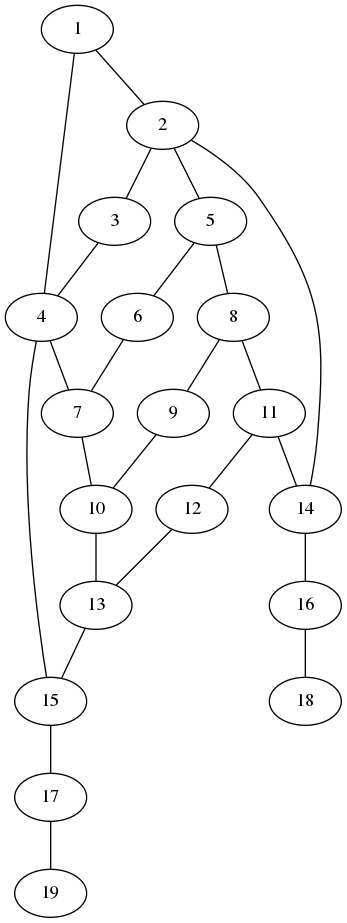
\includegraphics[scale=0.3]{figures/graph2.png}
  \caption{反例}
  \label{fig:label}
  \end{figure}

\begin{figure}[ht]
\centering
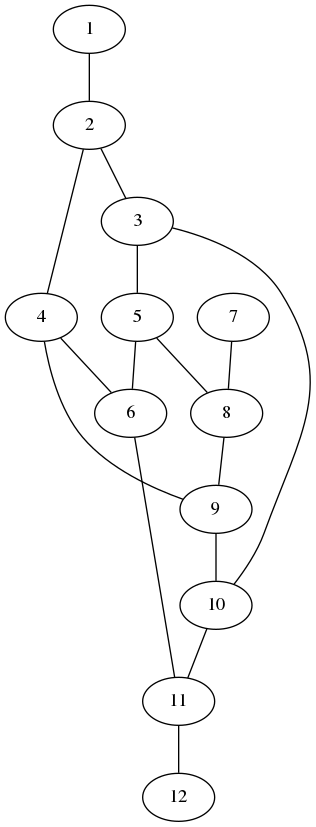
\includegraphics[scale=0.3]{figures/graph.png}
\caption{简单一些的反例}
\label{fig:label}
\end{figure}

\end{sol}
\end{problem}

\end{document}